\chapter{Implementation}
\label{chap:implementation}

This chapter describes the implementation steps to create a full text search. 
It is based on the designed index schema and Solr configuration described in Chapter \ref{chapter:indexDesign}.



% Text nize vyhodit

%Previous parts of the thesis shown that documents in index and records stored in relational database tables serve to different purposes and use cases and hence must be treated differently. 
% The treatment in this context means storing, structuring and saving the data.

%Being aware of the index structure and its specifics, it is almost always necessary to make a kind of transformation from the relational to the index form in order to make the full text search work properly and efficiently. 
%There are several ways to accomplish this goal, one of them involves flattening the relational structure. 
%This leads to denormalized data which is mostly unacceptable in relational databases, but since index is quite different from databases, denormalization is even desired. 
%The main thing one should know when designing an index structure is to know which search results a user expects and how the final representation of full text results should look like.
%
%If an approach of direct 1:1 mapping between entities and documents was chosen, the result would be a corresponding type of document for each entity. 
%The documents are expected to contain only a subset of fields the entities contain.

\section{Solr Spring Integration}
% ukazka, jak se vytvori instance solru pres beanu

To integrate Solr into the EEG/ERP Portal application, SolrJ API is used. 
In order to use the SolrJ API, it is needed to create a \texttt{SolrServer} class instance to enable communication with the remote Solr server. % from the application code.
This is why a Spring bean defining the \texttt{HttpSolrServer} instance was created in Spring application context, as shown in Listing \ref{listing:solrBeanConf}:

\begin{lstlisting}[language=XML, caption={Configuration of the Solr Server Bean.}, label={listing:solrBeanConf}]
<bean name="solrServer" class="org.apache.solr.client.solrj.impl.HttpSolrServer">
	<constructor-arg name="baseURL" value="${solr.serverUrl}"/>
	<property name="connectionTimeout" value="${solr.connectionTimeout}"/>
	<property name="defaultMaxConnectionsPerHost" value="${solr.defaultMaxConnectionsPerHost}"/>
  <property name="maxTotalConnections" value="${solr.maxTotalConnections}"/>
</bean>
\end{lstlisting}

\section{Indexing Data}

It was mentioned in Chapter \ref{chap:analysis} that it was needed to index data coming from different data sources.
Although the ways to build input Solr documents differ, the principle of indexing as the whole is the same for all data sources and can be divided into the following steps:

\begin{enumerate}
	\item A Solr document is created from input data.
	\item A connection between the Solr server and the EEG/ERP Portal application is established.
	\item The document is sent to the Solr server.
	\item Information about the created document is logged.
\end{enumerate}

It is obvious that the steps 2,3 and 4 are common for all kinds of data sources.
To separate common functionality of indexing from the specialized step during which a Solr document is built, the \textit{Template Method} design pattern \cite{GOF:DesignPatterns} was used.
By applying this design pattern, the class hierarchy depicted in Figure \ref{fig:indexersUml} was implemented.

\begin{figure}[h]
	\centering
		\includegraphics{figures/indexersUml.eps}
	\caption{UML Diagram of Indexer Classes}
	\label{fig:indexersUml}
\end{figure}

The parent abstract class \texttt{Indexer} takes care of performing the generic steps only by providing a \texttt{Http\-Solr\-Server} instance and implementing the \texttt{index()}, \texttt{index\-All()} and \texttt{log\-Commit\-Response()} methods, respectively. 
The step of document creation is handed over to its corresponding implementation of the \texttt{prepareForIndexing()} method  in one of the child classes.
There were three child classes (indexers) created, each being responsible for processing different input data:

\begin{itemize}
	\item \texttt{PojoIndexer} - indexer of POJO classes,
	\item \texttt{LinkedInIndexer} - indexer of LinkedIn articles,
	\item \texttt{AutocompleteIndexer} - indexer of searched phrases that improves the autocomplete functionality.
\end{itemize}

The following sections focus on the provided solutions to creating index documents from input data.
Therefore, three different implementations of the \texttt{prepareForIn\-de\-xing()} method in the classes listed above will be described.


\subsection{Database Indexing}

Generally speaking, the structure of data stored in RDBMS is not suitable for index of full text search engines.
The reasons behind this were already covered in Chapter \ref{chap:fulltext}.
Therefore, a transformation from relational data to document data had to be made.
The domain model and the related POJO classes and their fields of our interest were identified as well, in Chapter \ref{chap:analysis}, so as the expected output in a form of the created Solr schema fields. % which can be found in Chapter \ref{chap:analysis}, too.

\subsubsection{Possibilities of Indexing}
% Jak pomoci SolrJ zajistit v kombinaci s ostatnimi dostupnymi moznostmi integrace s EEG/ERP portalem

The first thing to solve is to choose the way of mapping the POJO fields into Solr schema fields.
By using the SolrJ API, it can be done by the following mechanisms:

\begin{itemize}
\item \textit{ \texttt{@Field} annotation} 
- The purpose of the \texttt{@Field} annotation is to mark the POJO fields that are to be indexed.
In combination with the \texttt{addBean()} and \texttt{addBeans()} methods provided by SolrJ API, Solr documents can be created.

However, this approach can be used only in a limited number of cases where a direct mapping of single-POJO fields is satisfactory.
In more advanced scenarios, such as mapping an object hierarchy to a Solr document, another alternative must be chosen. 
This limitation lies in the inability to use the \texttt{@Field} annotation to mark nested objects or object collections.

Furthermore, the usage of provided annotations brings a problem of ambiguity of mapped objects. 
Documents stored in the Solr index must possess an identifier which is unique across all stored documents. 
Object IDs are unique only in the class scope, so global uniqueness is not ensured. 

% (pouziti Solr UUID nebylo prostreleno). 

\item \textit{using the SolrJ's \texttt{addField()} method} - Although this alternative is not so comfortable as the previous one, it gives more control of creating a Solr document. 
This is because merging multiple POJOs into one Solr document can be achieved.
Nevertheless, using this method only would result in creating a less flexible code which is harder to maintain. 
%for object-document mapping separately cannot provide a universal solution to the given problem.


%\item \textit{aspects} 
%- Aspects are suitable for injecting so-called cross-cutting concerns such as logging and database transactions to avoid spreading the same lines of code across the whole application. 
%In our case, the existing need for indexing domain objects can be realized by simply enriching the base DAO methods responsible for creating, updating and deleting an object. 
%This way the indexing calls happen only in a few known places in code. 
%Introducing an extra aspect for this situation is more likely to be overkill, not to mention added complexity in debugging.

\item \textit{integration with Hibernate Search and using its annotation mechanisms}
 - The core idea of this proposed alternative is to use Hibernate Search capabilities, such as advanced indexing annotation support and automatic indexing of all collected changes, for the initial phase of indexing. 
Though it is possible to combine Hibernate Search and Solr (one of such ways to combine them can be found in \cite{HibSearch:CombinationSolr}), there would be an extra undesired dependency on another technology. 
% The future Hibernate Search version may change its API or some related internal implementation which may result in undesired bugs.
% Furthermore, there is a risk of potential negative side-effects created by this integration due to unsatisfactory analysis
%In addition, to cover indexing of data not present in RDBMS, other indexing mechanisms for these kinds of data would have to be 
% created anyway. 

\item \textit{custom annotation mechanism}
- By exploiting possibilities offered by Java Reflection and combining them with custom Java annotations, a universal solution covering all needs can be implemented.
This way, the problem of creating a Solr document from a class hierarchy, as well as the problem of the same document IDs, can be overcome. 
This alternative is undoubtedly the most challenging one, but its implementation can assure covering all specified needs. 
%gives more freedom than the previously proposed solutions. 

% one cannot be limited by the aforementioned solutions and create a new one that overcomes found problems. 
%It would be desirable to create a solution universal for all domain objects. 
%Inspired by the provided SolrJ annotations. 
% It also involves creating a custom code to implement generating a unique id for each created document.  

% NE! Patri ke zpusobum predavani do indexu
% \item filter - web.xml TODO custom filters

\end{itemize}

% Proc ted budeme mluvit o reflexi
%The last option best fits our needs from all those that are mentioned
For the above-mentioned reasons, it was decided to create a custom annotation mechanism for mapping POJO fields to their respective Solr document fields.
%Therefore, Java Reflection was frequently used to implement the new full text search solution. 
% Java Reflection will be described in the next few lines and its importance in the created code will be clarified.

\subsubsection{Java Reflection}
%Co to je, na co se pouziva, jak se pouziva v implementaci

% http://stackoverflow.com/questions/8392392/adding-to-a-list-via-reflection

% http://www.coderanch.com/t/383648/java/java/java-reflection-element-type-List

Java Reflection was frequently used to implement the new full text search solution. 
This is why its mechanism will be described in a few lines first.
Then, its usage throughout the created code of full text search will be demonstrated.

\subsubsection{Introducing Java Reflection}

Reflection is the ability to inspect the code and make its modifications at runtime. 
It is a feature that makes staticly-typed languages like Java more dynamic. 
Its heavy usage can be found especially in modern frameworks such as Spring or Hibernate, that both use reflection for instantiating classes from information in configuration files. 

A very common use case of reflection in Java is the usage with annotations. 
This combination opens many possibilities of manipulating class metadata. 
In \textit{JUnit 4}, for example, the \texttt{@Test} annotation was introduced. 
The JUnit framework looks up all methods marked by this marker annotation and call them in each execution of running unit tests.

The root class of the Java object hierarchy, the Object class, has the \texttt{getClass()} method providing the corresponding \texttt{Class} object, meaning that all Java classes can be invoked or inspected by means of reflection.

% \subsubsection{Usage of Java Reflection in the EEG/ERP Portal}
% dat priklady, asi i vcetne kodu


%
%The name reflection is used to describe code which is able to inspect other code in the same system (or itself).
%
%One very common use case in Java is the usage with annotations. JUnit 4, for example, will use reflection to look through your classes for methods tagged with the @Test annotation, and will then call them when running the unit test.
%
 %The ability to inspect the code in the system and see object types is Type Introspection. Reflection is then the ability to make modifications at runtime by making use of introspection.
%
 %For example, all objects in Java has the method getClass, which lets you determine its class even if you don't know it at compile time (like if you declared it as Object) - this might seem trivial, but such reflection is not by default possible in less dynamic languages such as C++.
%
%Take for example your typical web.xml file. This will contain a list of servlet elements, which contain nested servlet-class elements. The servlet container will process the web.xml file, and create new a new instance of each servlet class through reflection.
%
%Reflection is important since it lets you write programs that does not have to "know" everything at compile time, making them more dynamic, since they can be tied together at runtime. The code can be written against known interfaces, but the actual classes to be used can be instantiated using reflection from configuration files.
%
%Lots of modern frameworks uses reflection extensively for this very reason. the most comprehensive example is Spring which uses reflection to create its beans, and for its heavy use of proxies
%
%It's useful in a lot of situations. Everywhere you want to be able to dynamically plug in classes into your code. Lot's of object relational mappers use reflection to be able to instantiate objects from databases without knowing in advance what objects they're going to use. Plug-in architectures is another place where reflection is useful. Being able to dynamically load code and determine if there are types there that implement the right interface to use as a plugin is important in those situations.

\subsubsection{Annotation Interface}

In order to inspect classes and collect required field values, the classes as well as the some of the fields within them need to be marked by annotations.
Three different annotations serving different purposes were created:

\begin{itemize}
	\item \texttt{@Indexed} - both class (type) and field annotation that can be used in two ways: When it is used to annotate classes, it marks the parent POJO classes; when used on the field level, it marks child POJO classes or their collections,
	\item \texttt{@SolrField} - a field annotation which marks the fields whose values should be contained in a Solr document,
	\item \texttt{@SolrId} - a field annotation that determines the fields belonging to the unique identifier of indexed classes.
\end{itemize}

Listing \ref{listing:annotationIfaceExample} provides an example of creating the \texttt{@SolrField} field annotation. 
Note that this annotation has the \texttt{name} attribute which serves to specify the matching field name in the Solr schema.
All used Solr field names are defined as enumeration constant values of the \texttt{IndexField} class/enumeration to avoid mistyping them.

\begin{lstlisting}[language=Java, caption={Example of Creating the \texttt{@SolrField} Annotation.}, label={listing:annotationIfaceExample}]
@Target(ElementType.FIELD)
@Retention(RetentionPolicy.RUNTIME)
public @interface SolrField {
    IndexField name();
}
\end{lstlisting}

The usage of the defined annotations is demonstrated on the code of the \texttt{Experiment} class in Listing \ref{listing:annotatedClassExample} (irrelevant lines are omitted). 
It is worth noting that the associated POJO collections, whose fields logically belong to the same Solr document, are annotated accordingly.

\begin{lstlisting}[language=Java, caption={Example of Using Indexing Annotations in the \texttt{Experiment} Class.}, label={listing:annotatedClassExample}]
@Indexed 
public class Experiment implements Serializable {
	@SolrId
	private int experimentId;
	@Indexed
	private Weather weather;
	@SolrField(name = IndexField.TEMPERATURE)
	private int temperature;
	@SolrField(name = IndexField.TEXT)
	private String environmentNote;
	@Indexed
	private Set<Hardware> hardwares = new HashSet<Hardware>(0);
	@Indexed
	private Set<Pharmaceutical> pharmaceuticals = new HashSet<Pharmaceutical>(0);
	@Indexed
	private Set<Disease> diseases = new HashSet<Disease>(0);
	@Indexed
	private Set<Software> softwares = new HashSet<Software>(0);
	...
}
\end{lstlisting}

The first practical application of Java Reflection discussed in this text is strongly related to the created set of annotations.
To leverage the semantics hidden behind the used annotations, it is necessary to use reflection to introduce indexing logic by inspecting these annotated classes.

\subsubsection{Indexing Algorithm}

In the \texttt{prepareForIndexing()} method, it is first found out if the type of a given \texttt{Object} instance, sent as the method parameter, has the \texttt{@Indexed} annotation assigned.
If it does, it can continue traversing the class fields by searching a field with the \texttt{@SolrId} annotation.
The value of such annotated field is used for assembling Solr document fields for later identification of a document.
These document fields were described in Chapter \ref{chapter:indexDesign}.

The next step of the algorithm is of recursive nature and happens on two levels - on the parent and the child level.
In both cases, all values of those fields containing the \texttt{@SolrField} annotation are extracted.
On the parent level, in addition, the fields with the \texttt{@Indexed} annotation are searched to identify the associated child \texttt{Collection} or \texttt{Object} classes which are then traversed.

% The values obtained from the collections are stored in 

The schema in Figure \ref{fig:indexAlgorithm} visually depicts the main idea of the described algorithm.

%TODO
%ma to na starosti metoda prepareForIndexing, ktera si jako parametr bere Object instanci (viz template figure vyse).
%Nejprve se zjisti, zda ma jeho trida prirazenu anotaci @Indexed.
%V kladnem pripade se zjisti, jestli nektery jeji field ma anotaci @SolrId.
%Z hodnoty tohoto fieldu jsou sestaveny document fieldy pro identifikaci dokumentu, ktere byly popsany v kapitola index design.
%Jsou take znazorneny na obrazku indexovaciho algoritmu.
%Pak dochazi k extrakci hodnot vsech fieldu , ktere maji anotaci @SolrField.
%Deje se tak na dvou urovnich - na urovni rodice a na urovni potomku obsazenych v asociovanych objectech nebo kolekcich.
%Nejdrive se prohledava na urovni rodice.
%Krome fieldu s anotaci @SolrField se take prohledavaji ty fieldy s anotaci @Indexed.
%Pro kolekce a objekty takto anotovane


\begin{figure}[h]
	\centering
		\includegraphics[width=1.00\textwidth]{figures/indexAlgorithm.eps}
	\caption{POJO Indexing Algorithm Schema.}
	\label{fig:indexAlgorithm}
\end{figure}


%All objects annotated by the @Indexed annotation represent the target objects which are required to be searched on.
%Apart from their own object fields, such as title or description of the Scenario object, these objects also contain associated collections of other objects. The fields of objects in the collections need to be indexed as well, since they are related to their respective parent objects. Furthermore, data contained in these nested objects are useful for users to look up required information by using the full text search.

%The conversion of this object structure to the corresponding document in the index is therefore not a straightforward task.
%A transformation from one structure to another must be done.
%If the object structure was flat and there were no associations among the objects, the transformation would be relatively easy to do. In case of independence of all objects, the only thing necessary to do would be to provide a way to determine which fields should be a part of the Solr document, thus to be make searchable.

%Using this approach has some serious disadvantages. 
%It breaks object associations, so it keeps objects separated (isolated).
%Its actual implementation turns out to be quite easy since no additional mapping or traversal needs to be done. 
%Nevertheless, all information which is logically bound to the table record in a form of associations on the database level and in a form of object references on the object level are lost.


\subsubsection{Ensuring eager loading}

In order to make the indexing algorithm work, associated POJO collections, whose object field values are desired to be indexed, have to be already initialized.
This condition, however, is not always met.
As written earlier in Chapter \ref{chap:eegPortal}, it is desired to apply lazy loading of object collections for as many cases as possible. If it is necessary, switching to the eager loading strategy can be done using the following ways:

\begin{itemize}
	\item{change of Hibernate mapping configuration}
	- This modification involves setting the \texttt{lazy=''false''} attribute for collections to be eagerly loaded. 
	It means that all affected 1:N relationships are always loaded together with the parent object. 
	This approach is not very flexible, because no proxies are created and the lazy loading behavior cannot be therefore configured at runtime.

	\item {custom HQL queries or Hibernate criteria that force eager fetching}
	- If HQL queries are used, one can specify eager fetching using the \texttt{fetch} keyword. 
	In case of using the Criteria Query API, the \texttt{setFetchMode()} method with its fetch mode attribute set to \texttt{FetchMode.EAGER} does the job.
	This alternative is more flexible than the previous one since lazy object initialization, which is set by default, is overridden by the eager fetch mode. 
	The created proxy objects call the associated real objects to fetch necessary data. 
	The drawback of this solution is the necessity to create custom HQL queries or Hibernate criteria for each entity that will cause collections to be lazy-loaded. As the created queries can differ a lot, it is very difficult to apply this solution in a generic way.
	

	\item {usage of the \texttt{Hibernate.initialize()} method} 
		- This method is used to initialize lazy-loaded collections. Its parameter takes an object that is to be fetched to the parent object.
		The method also ensures that all already initialized objects will be omitted.
		The power of the \texttt{Hibernate.initialize()} method lies in its universality. When used together with Java Reflection, a universal solution enforcing eager loading of collections for any POJO object can be achieved. 
		It can be used even after the session is closed.

\end{itemize}


Based on the aforementioned possibilities and current requirements, using the \texttt{Hibernate.initialize()} method in combination with the power of Java Reflection was preferred. 

This decision leads to modification of the \texttt{SimpleGenericDao} class. It was enriched of a new generic method which implements the chosen eager loading strategy. 
The method, namely the \texttt{getAllRecordsFull()} method, works on the principle of finding out all proxied object fields, i.e. those fields which are not initialized yet.
All fields are accessed by reflective calls of their respective getter methods available in a given class.
The fields are then initialized by adding them as the parameters of subsequent \texttt{Hibernate.initialize()} method calls.

The following Listing \ref{listing:eagerByReflection} shows the implementation of eager loading on demand described in the paragraph above.

% Dat kod te metody do prilohy?
\begin{lstlisting}[language=Java, caption={Enforcing Eager Loading by Using Java Reflection.}, label={listing:eagerByReflection}]
public List<T> getAllRecordsFull() {
	List<T> records = getAllRecords();
	for(T record : records) {
		Method[] methods = record.getClass().getDeclaredMethods();
    for (Method method : methods) {
			if(method.getName().startsWith("get") && !method.getReturnType().isPrimitive()) {
				try {
					initializeProperty(method.invoke(record));
        } catch (IllegalAccessException e) {
					log.error(e);
        } catch (InvocationTargetException e) {
					log.error(e);
        } catch (Exception e) {
					log.error(e);
        }
      }
    }
  }
  return records;
}

...

protected void initializeProperty(Object property) {
	if(!Hibernate.isInitialized(property)) {
		getHibernateTemplate().initialize(property);
  }               
}
\end{lstlisting}



\subsection{LinkedIn Indexing}

% The following text uses 

% dat spis do teorie !!!
%\subsubsection{REST}
%
%leverages existing technologies - HTTP GET update - POST or PUT. It has taken the advantage of the HTTP protocol itself to describe the action that should be performed on a given resource.

\subsubsection{Using Spring Social}
% Proc primy vyuziti nestaci, jak vyresit, priklad, co se implementovalo

The methods provided by Spring Social are set to give a user a set of default fields that are appropriate for some use cases. 
Although it is very convenient to have such layer of abstraction, sometimes there is a need to obtain other fields or to omit some of them. 
For example, if the Spring Social method for getting all articles in a group is called, some information, such as article summaries and their time stamps, are missing. 
In such cases, a custom LinkedIn REST call must be created and put as a parameter of the \texttt{restOperations().getForObject()} method provided by Spring Social.
The call can contain field selectors which are used to specify which fields to return in the response.
The following example in Listing \ref{listing:linkedinRest} shows the usage of field selectors in the REST call.
The REST call in the listing gets full information about twenty latest LinkedIn articles published in the EEG/ERP Portal group.
Note the \texttt{{group-id}} placeholder which is later substituted by the real value of the EEG/ERP Portal group ID.

%Group.GroupPosts groupPosts = linkedin.restOperations().getForObject(
	%"http://api.linkedin.com/v1/groups/{group-id}/posts" +
  %":(creation-timestamp,title,summary,id," +
  %"creator:(first-name,last-name))?" +
  %"count=" + count +
  %"&start=" + start +
  %"&order=recency",
  %Group.GroupPosts.class, groupId);
%return groupPosts.getPosts();

\begin{lstlisting}[language=HTML, caption={Example of a LinkedIn REST API call.}, label={listing:linkedinRest}]
http://api.linkedin.com/v1/groups/{group-id}/posts:
(creation-timestamp,title,summary,id,creator:(first-name,last-name))?
count=20&start=0&order=recency"

\end{lstlisting}

In the application code, LinkedIn REST calls are wrapped in the methods of the \texttt{LinkedInManager} class. The class includes these methods using direct LinkedIn REST calls:

\begin{itemize}
	\item \texttt{getGroupPostsWithMoreInfo(int count, int start)} - It uses a very similar REST call as the one in Listing \ref{listing:linkedinRest} to obtain LinkedIn articles. 
	The number of retrieved articles and the index position of the first retrieved articles are defined in the method parameters. 
	% \item \texttt{getLastPost()} - This method returns the last post added to the EEG Portal LinkedIn group.
	% \item \texttt{getLastPostId()} - Returns the id value of the last post added to the EEG Portal LinkedIn group.
	\item \texttt{getPostById(String id)} - Gets a LinkedIn post by its unique ID.
	\item \texttt{deletePost(String id)} - Deletes a post by specifying its ID as the method parameter.
\end{itemize}

Apart from the methods mentioned above, the following methods were added to the \texttt{LinkedInManager} class as well:
% jsou pouzity ve spojeni s indexovanim

\begin{itemize}
	\item \texttt{getLastPost()} - This method returns the last post added to the EEG Portal LinkedIn group.
	\item \texttt{getLastPostId()} - Returns the id value of the last post added to the EEG Portal LinkedIn group.
\end{itemize}

Usage of these methods is related to indexing LinkedIn articles which are created by using the EEG/ERP Portal.

\subsubsection{Article-document Mapping}

Compared to POJO-document mapping, mapping from the LinkedIn article to the created Solr document structure is straightforward.
Received LinkedIn Post objects store only unique string ID, article title and summary values, so converting them to Solr documents involves copying these values to the respective \texttt{uuid}, \texttt{text} and \texttt{title} document fields.
Apart from that, the document fields \texttt{class} and \texttt{source} must be populated in order to find these articles successfully while doing a full text search.


\subsection{Indexing Searched Phrases}
% proc vubec a jak implementovano

It was decided to make searched phrases indexable.
Indexing them enables the phrases to appear in the autocomplete box.
Moreover, by indexing search phrases, search frequency of each phrase can be found out and stored together with the phrase in the document.
This way, indexed phrase frequencies enable suggesting the most queried phrases first.

Internally, a phrase and its search frequency are stored together in the \texttt{autocomplete} Solr field and are separated by the number sign (\#) symbol.

\subsection{Changing Indexed Data}

When some data stored in RDBMS are removed or edited, the made changes need to be reflected in the Solr index.
In case if parent POJO objects are changed, the analogous document changes can be performed by using the indexer's \texttt{index()} and \texttt{unindex()} methods. The first method simply overwrites a stored document having the same \texttt{uuid} field as the new inserted one. The latter method removes a document determined by an object set as the method parameter.

However, child objects have no direct document equivalents, because they form only a part of the documents of parent objects.
Although partial updates are possible since Solr 4.0, they are not implemented.
The reasons of not implementing them are the following:
	
	\begin{itemize}
		\item It is expected that the EEG/ERP Portal application is designed to treat the child objects always in the context of their parent object.
		\item Adding the partial update support brings a new level of complexity into the application. Due to the application nature and its requirements, the added complexity was not worth the effort in this case.
	\end{itemize}

Nevertheless, if a change of a child object happens, the index will become inconsistent.	
This is why periodic indexing of database data has to be ensured to prevent potential inconsistent index states and to reach the so-called \textit{eventual consistency}.

Almost the same applies to LinkedIn articles where the problem is extended by adding, updating and removing the articles by the means of the LinkedIn website. 

\subsection{Periodic indexing}

\subsubsection{LinkedIn Articles}
There are two ways to add an article to the EEG/ERP Portal group: either indirectly by filling in the form on the EEG/ERP Portal website or directly from LinkedIn.

In the first case, articles can be indexed immediately after publishing them because their times of publishing are known due to the interaction with the EEG/ERP Portal. 
The last published article in the LinkedIn group can be fetched by the means of LinkedIn REST API and then modified by the indexer so that information about the article can be added to the index.

The latter case is more complicated as there is no interaction with the EEG/ERP Portal. 
So in order to index all LinkedIn articles, the article data must be retrieved first.
It can be done by using LinkedIn REST API calls to receive their object representation.
Since there is no available information of when articles are uploaded to LinkedIn, the REST calls must be done periodically.
This way, periodic indexing of all articles published on LinkedIn can be achieved.

Although the obvious disadvantage of periodic indexing is the existence of a delay between publishing times of some articles and their indexing times (which is equal to the indexing period in the worst case), this method assures that all articles get indexed in the end.

\subsubsection{Scheduling in Spring}

% http://javahunter.wordpress.com/2011/05/05/cronscheduler-in-spring/

The Spring Framework has a native support of task scheduling and asynchronous calls. 
Since its version 3.0, methods can be scheduled and also run asynchronously by using annotations, namely the \texttt{@Scheduled} and \texttt{@Async} annotations. 
The first mentioned annotation, when added to a method, makes the method schedulable by Spring. 
Usage of this annotation is restricted to the void methods with no parameters. 
The \texttt{@Scheduled} annotation has to contain a piece of metadata to tell Spring how to plan the method scheduling. 
Currently there are three available attributes for the \texttt{@Scheduled} annotation, from which the most flexible option is specifying a cron expression to trigger a task as shown on the following lines:

\begin{lstlisting}[language=Java, caption={Example of a Cron Expression.}, label={listing:cronExpression}]]
@Scheduled(cron=* 0 22 * * SAT-SUN)
public void indexAll()
\end{lstlisting}


This way, the method \texttt{indexAll()} will be scheduled to run always at 10 pm only on Saturdays and Sundays. 
The cron syntax allows a user to create more sophisticated scheduling scenarios, but discussing the syntax is out of scope of this work. 
Since Spring is internally using Quartz as a scheduler, an interested reader can find all necessary information about the syntax in the Quartz documentation \cite{QuartzDoc}.

The \texttt{@Async} annotation is used to mark the methods to be invoked asynchronously.
It is very easy to use for methods having void return values.
Listing \ref{listing:asyncAnnotation} shows the usage of the \texttt{@Async} annotation for the \texttt{indexLinkedIn()} and \texttt{indexDatabase()} methods that handle LinkedIn-articles and RDBMS indexing, respectively.


\begin{lstlisting}[language=Java, caption={Using the \texttt{@Async} Annotation.}, label={listing:asyncAnnotation}]
@Async
public void indexLinkedIn()
...
@Async
public void indexDatabase()
\end{lstlisting}

In order to enable annotation-based scheduling, it is necessary to add a new element in the application context file as well as the \texttt{task} namespace to which the element belongs (see Listing \ref{listing:springTaskNs}).

\begin{lstlisting}[language=XML, caption={Using task namespace}, label={listing:springTaskNs}]
<xmlns:task="... http://www.springframework.org/schema/task" 
xsi:schemaLocation="... http://www.springframework.org/schema/task/spring-task.xsd">
...
<task:annotation-driven executor="indexingExecutor" scheduler="indexingScheduler"/>
\end{lstlisting}

The annotation-driven element requires \texttt{executor} and \texttt{scheduler} attributes to be set to handle tasks represented by methods marked by \texttt{@Async} and \texttt{@Scheduled} annotations, respectively.
The related lines can be seen in Listing \ref{listing:settingSpringExecSched}:

\begin{lstlisting}[language=XML, caption={Setting Spring Executer and Scheduler.}, label={listing:settingSpringExecSched}]
<task:executor id="indexingExecutor" pool-size="5"/> 
<task:scheduler id="indexingScheduler" pool-size="1"/>
\end{lstlisting}


%
%,,Notice that an executor reference is provided for handling those
%tasks that correspond to methods with the @Async annotation, and the
%scheduler reference is provided for managing those methods annotated
%with @Scheduled.``

	
\subsection{UML Class Diagram}

The relationships among classes that create the indexing part of the full-text search are depicted in Figure \ref{fig:umlDiagramIndexing}.

\begin{figure}[h]
	\centering
		\includegraphics[width=1.00\textwidth]{figures/diagram_indexing.png}
	\caption{UML Class Diagram of the Indexing Part.}
	\label{fig:umlDiagramIndexing}
\end{figure}

There can be seen these most important classes:

\begin{itemize}
	\item \texttt{IndexingService} - Contains the indexing methods \texttt{indexDatabase()} and \texttt{indexLinkedIn()} described above that handle periodic indexing.
	\item \texttt{Indexer} - Direct usage of its \texttt{index()} and \texttt{unindex()} methods is made when any of POJO objects or LinkedIn \texttt{Post}s is created, updated or deleted. Thus every domain object must be associated with its indexing in the first two cases and its removal from the index in the last case. It is achieved by calling these methods in the \texttt{create()}, \texttt{update()} and \texttt{delete()} in the \texttt{Simple\-Gene\-ric\-Dao} class and in the \texttt{publish} and \texttt{deletePost} methods of the \texttt{Linked\-In\-Ma\-na\-ger} class.
\end{itemize}

	
\section{Searching}

This section deals with the search user interface.
The interface was implemented by using the Wicket Framework.

% byly vytvoreny komponenty, ktere byly do sebe vnorovany
% hlavni logika vyhledavani je obsazena ve tride FulltextSearchService

\subsection{Search Logic}

Most of the search logic can be found in the \texttt{FulltextSearchService} class.
This method is responsible for: 

\begin{itemize}

	\item returning search results for a given query - method \texttt{getResults\-ForQuery()}
	\item returning suggested search phrases for autocomplete - method \texttt{getText\-To\-Auto\-complete()}
	\item returning a total number of found documents for a given query - method \texttt{getTotal\-NumberOf\-Documents\-ForQuery()}
	\item faceting by document categories - method \texttt{get\-Category\-Fa\-cets(String solrQuery)}

\end{itemize}

The method \texttt{getResultsForQuery} returns \texttt{FullTextResult} objects that represent results received from the Solr server for a query.
The \texttt{FullTextResult} class, in fact, contains fields that match those contained in the Solr document, i.e. the fields whose information has a value for users - document title, text fragments with highlighted searched keywords, type of the document, class of a Wicket target page which contains further details, id of a corresponding POJO, and time of indexation.

\subsection{Full-text Search User Interface}

Objects of the \texttt{FullTextResult} class are handed over to classes that form the full-text search user interface.  

Namely, these classes include:

\begin{itemize}
	
	\item \texttt{SearchFacets} - It creates faceted search by showing number of found results for each of the document categories, allowing to filter the found results by the document category. Uses the \texttt{FacetCategory} class - name, count, and enumeration \texttt{ResultCategory}. % TODO
	
	\item \texttt{SearchPanel} - This abstract class represents a search panel that provides all necessary functionality, including the autocomplete capability. 
The reason why the class is abstract is that Wicket enforces to have a separate class for each HTML markup. 
Since it is required to have one search panel in the page header and another one, which is different by appearance, in the search page, their corresponding classes had to be created.
There is the \texttt{MenuSearchPanel} class for the search panel located in the page header. For displaying the search panel in the search page, the \texttt{PageSearchPanel} class was made.
	
	\item \texttt{SearchResultPanel} - It is responsible for displaying search results. % which are populated to the Wicket \texttt{DataView} component. 
	The search results are rendered by using the created \texttt{Search\-Result\-Data\-Provider} class that communicates with the \texttt{Fulltext\-Search\-Ser\-vice} class to obtain the matching \texttt{FullTextResult} instances. Besides that, it also displays the number of found results per each document category by utilizing an instance of \texttt{SearchFacets}.
	
	\item \texttt{SearchPage} - It represents the search page. It uses the listed \texttt{Search\-Re\-sult\-Pa\-nel} and \texttt{Page\-Search\-Panel} classes to display necessary information. 
	
\end{itemize}


% \subsection{Handling synonyms}
%  jak konfigurovat, moznosti, ukazka --> DAT DO INDEX DESIGN
%  nevyhody defaultniho reseni v Solru, jak je mozno vylepsit --> DAT DO INDEX DESIGN

% http://stackoverflow.com/questions/4493140/how-to-reload-synonyms-txt-in-solr

% http://nolanlawson.com/2012/10/31/better-synonym-handling-in-solr/

% http://www.quora.com/Apache-Solr/How-can-I-load-the-synonyms-words-from-MySQL-in-Solr


%\subsection{Search Results}

\subsection{UML Class Diagram}

The described classes related to searching documents and associations among them are depicted in the UML class diagram in Figure \ref{fig:umlDiagramSearching}

\begin{figure}[h]
	\centering
		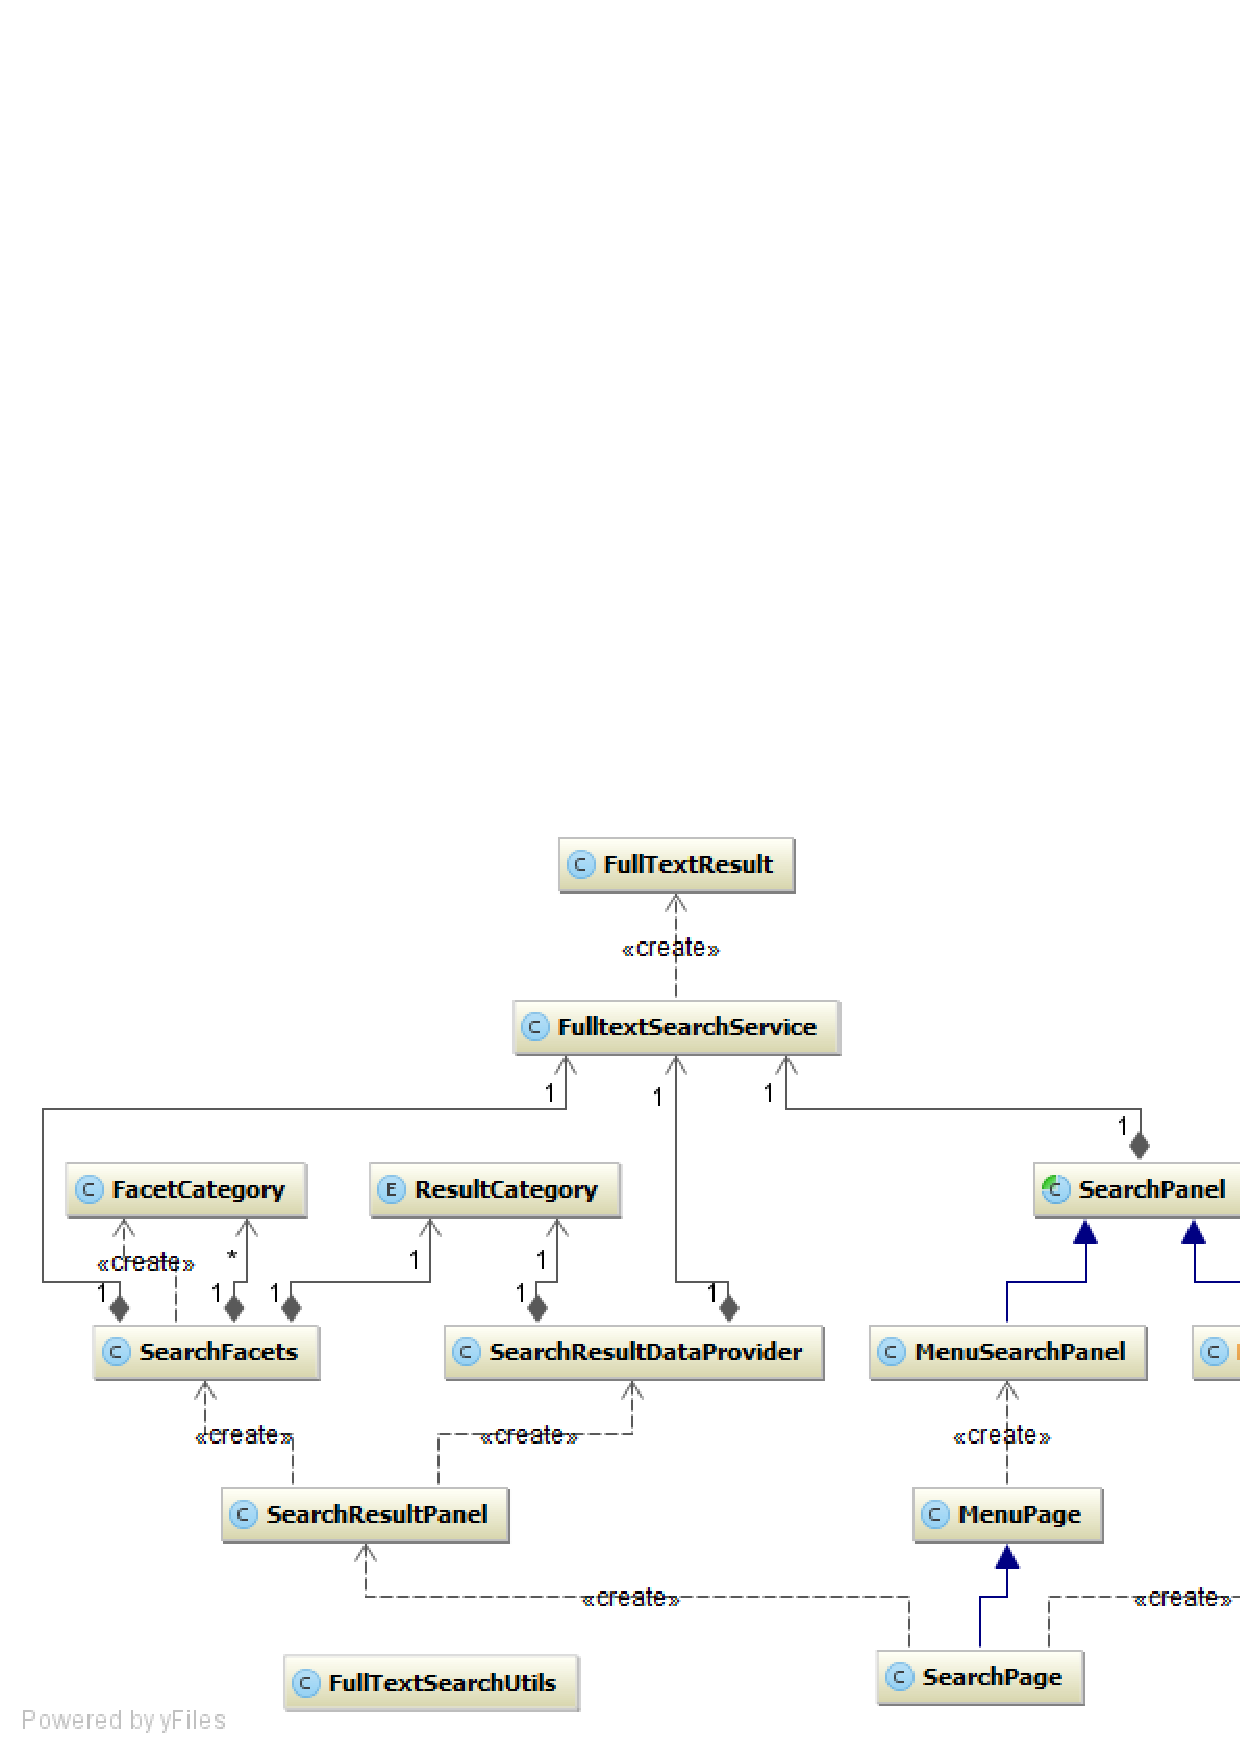
\includegraphics[width=1.00\textwidth]{figures/diagram_search.png}
	\caption{UML Class Diagram of the Search Part.}
	\label{fig:umlDiagramSearching}
\end{figure}

%\subsection{Search Form}

%\subsubsection{Autocomplete}

%\subsubsection{Highlighting}

%\subsubsection{Faceting}

% http://searchhub.org/2009/09/02/faceted-search-with-solr/

% http://lucene.472066.n3.nabble.com/Highlighting-in-SolrJ-td495857.html

% http://www.optimation.co.nz/optimation-blog/01-03-2011/open-source-faceted-searching-using-solr-and-solrj


